

\documentclass[DM,authoryear,toc]{lsstdoc}
% lsstdoc documentation: https://lsst-texmf.lsst.io/lsstdoc.html

% Package imports go here.

% Local commands go here.

% To add a short-form title:
% \title[Short title]{Title}
\title{S17B HSC PDR1 Reprocessing Report}

% Optional subtitle
% \setDocSubtitle{A subtitle}

\author{%
Hsin-Fang Chiang, Greg Daues, Samantha Thrush, and the NCSA team
}

\setDocRef{DMTR-31}

\date{\today}

% Optional: name of the document's curator
% \setDocCurator{The Curator of this Document}

\setDocAbstract{%
This document captures information about the large scale HSC reprocessing we performed in Cycle S17B.
}

% Change history defined here.
% Order: oldest first.
% Fields: VERSION, DATE, DESCRIPTION, OWNER NAME.
% See LPM-51 for version number policy.
\setDocChangeRecord{%
  \addtohist{1}{YYY-MM-DD}{Unreleased.}{Hsin-Fang Chiang}
}

\begin{document}

% Create the title page.
% Table of contents is added automatically with the "toc" class option.
\maketitle

% ADD CONTENT HERE
\section{Dataset Information}
The input dataset is the HSC Strategic Survey Program (SSP) Public Data Release 1 (PDR1) \citep{2017arXiv170208449A}.
The PDR1 dataset has been transferred to the LSST GPFS storage /datasets by \jira{DM-9683} and the butler repo is available at /datasets/hsc/repo.

It includes 5654 visits in 7 bands: HSC-G, HSC-R, HSC-I, HSC-Y, HSC-Z, NB0816, NB0921. A file including all visit IDs is attached to the confluence page.  The official release site is at https://hsc-release.mtk.nao.ac.jp/
The survey has three layers and includes 8 fields.
\begin{enumerate}
\item
UDEEP: SSP{\_}UDEEP{\_}SXDS, SSP{\_}UDEEP{\_}COSMOS
\item
DEEP: SSP{\_}DEEP{\_}ELAIS{\_}N1, SSP{\_}DEEP{\_}DEEP2{\_}3, SSP{\_}DEEP{\_}XMM(S){\_}LSS, SSP{\_}DEEP{\_}COSMOS
\item
WIDE: SSP{\_}WIDE, SSP{\_}AEGIS
\end{enumerate}

The number of visits in each field and band is summarized in \tabref{tab:dataset}.

%Summary of the input dataset
\begin{tabular}{lllllllll}
& & HSC-G & HSC-R & HSC-I & HSC-Z & HSC-Y & NB0921 & NB0816  \\
Layer & Field Name ("OBJECT") & \multicolumn{7}{c}{Number of visits} \\
DEEP & SSP{\_}DEEP{\_}ELAIS{\_}N1 & 32&24&28&51&24&20&0 \\
DEEP & SSP{\_}DEEP{\_}ELAIS{\_}N1 &32&24&28&51&24&20&0 \\
DEEP & SSP{\_}DEEP{\_}DEEP2{\_}3 &32&31&32&44&32&23&17 \\
DEEP & SSP{\_}DEEP{\_}XMM{\_}LSS &25&27&18&21&25&0&0 \\
DEEP & SSP{\_}DEEP{\_}COSMOS &20&20&40&48&16&18&0 \\
UDEEP&SSP{\_}UDEEP{\_}SXDS&18&18&31&43&46&21&19 \\
UDEEP & SSP{\_}UDEEP{\_}COSMOS&19&19&35&33&55&29&0 \\
WIDE&SSP{\_}AEGIS&8&5&7&7&7&0&0 \\
WIDE & SSP{\_}WIDE&913&818&916&991&928&0&0 \\
\end{tabular}


The tract IDs for each field, obtained
from https://hsc-release.mtk.nao.ac.jp/doc/index.php/database/
is summarized in \tabref{tab:tractIds}.

%Summary of the input dataset
\begin{tabular}{lll}
Layer & Field Name ("OBJECT") & Tract IDs \\
DEEP & SSP{\_}DEEP{\_}ELAIS{\_}N1 & 16984, 16985, 17129, 17130, 17131, 17270, 17271, 17272, 17406, 17407 \\
DEEP & SSP{\_}DEEP{\_}DEEP2{\_}3 & 9220, 9221, 9462, 9463, 9464, 9465, 9706, 9707, 9708 \\
DEEP & SSP{\_}DEEP{\_}XMM{\_}LSS & 8282, 8283, 8284, 8523, 8524, 8525, 8765, 8766, 8767 \\
DEEP & SSP{\_}DEEP{\_}COSMOS & 9569, 9570, 9571, 9572\footnote{tract 9572 is listed on HSC PDR1 website for DEEP{\_}COSMOS but no data actually overlap it; PDR1 does not have it either.}, 9812, 9813, 9814, 10054, 10055, 10056 \\
UDEEP&SSP{\_}UDEEP{\_}SXDS& 8523, 8524, 8765, 8766 \\
UDEEP & SSP{\_}UDEEP{\_}COSMOS& 9570, 9571, 9812, 9813, 9814, 10054, 10055 \\
WIDE&SSP{\_}AEGIS& 16821,16822, 16972, 16973 \\
\multirow{3}{*}{WIDE} & \multirow{3}{*}{SSP{\_}WIDE}
& XMM: 8279-8285, 8520-8526, 8762-8768 \\
&&GAMA09H: 9314-9318, 9557-9562, 9800-9805 \\
&&WIDE12H: 9346-9349, 9589-9592 \\
&&GAMA15H: 9370-9375, 9613-9618 \\
&&HECTOMAP: 15830-15833, 16008-16011 \\
&&VVDS: 9450-9456, 9693-9699, 9935-9941 \\
\end{tabular}


Plots of tracts and patches can be found on  \url{https://hsc-release.mtk.nao.ac.jp/doc/index.php/data/}. In S17B, processing of some edge tracts not listed in \tabref{tab:tractIds} was attempted and those data were not removed from the output repos. Those data can be ignored; see \ref{summaryOutputs}.

\section{Hardware}
The processing was done using the Verification Cluster.
The Verification Cluster consists of 48 Dell C6320 nodes with 24 physical cores (2 sockets, 12 cores per processor) and 128 GB RAM. As such, the system provides a total of 1152 physical cores.
lsst-dev01 is a system with 24 physical cores, 256 GB RAM, running the latest CentOS 7.x that serves as the front end of the Verification Cluster.

The Verification Cluster runs the Simple Linux Utility for Resource Management (SLURM) cluster management and job scheduling system. lsst-dev01 runs the SLURM controller and serves as the login or head node , enabling LSST DM users to submit SLURM jobs to the Verification Cluster.

lsst-dev01 and the Verification Cluster utilize the General Parallel File System (GPFS) to provided shared-disk across all of the nodes. The GPFS will have spaces for archived datasets and scratch space to support computation/analysis.



\section{Software}

The LSST software stack is used. A shared software stack on the GPFS file systems, suitable for computation on the Verification Cluster, has been provided and is maintained by Science Pipelines and is available under /software/lsstsw.

The stack version of $w{\_}2017{\_}17$, published on 26-Apr-2017, was used.
Besides, the master branch of $meas{\_}mosaic$, $obs{\_}subaru$, and $ctrl{\_}pool$ from 7-May-2017 and built with $w{\_}2017{\_}17$ was used.
This is equivalent to the week 17 tag with \jira{DM-10315}, \jira{DM-10449}, and \jira{DM-10430}.

Unless otherwise noted, the HSC default config in the stack is used, including the task defaults and $obs{\_}subaru$'s overrides.
That implies the PS1 reference catalog $ps1{\_}pv3{\_}3pi{\_}20170110$ in the LSST format (HTM indexed) is used (/datasets/refcats/htm/ps1{\_}pv3{\_}3pi{\_}20170110/).
The calibration dataset is the 20170105 version from Paul Price; the calibration repo is located at /datasets/hsc/calib/20170105 from \jira{DM-9978}.
The externally provided bright object masks (butler type "brightObjectMask") of version "Arcturus" (\jira{DM-10436}) are added to the repo and applied in coaddDriver.assembleCoadd.

\subsection{Pipeline steps and configs}
\begin{enumerate}
\item
makeSkyMap.py
\item
singleFrameDriver.py
\begin{enumerate}
\item [-]
Note: Ignore ccd=9 which has bad amps and results not trustworthy even if processCcd passes
\end{enumerate}
\item
mosaic.py
\item
coaddDriver.py
\begin{enumerate}
\item [-]
Note: Make config.assembleCoadd.subregionSize small enough so a full stack of images can fit into memory at once; a trade-off between memory and i/o but doesn't matter scientifically, as the pixels are independent.
\end{enumerate}
\item
multiBandDriver.py
\item
forcedPhotCcd.py
\begin{enumerate}
\item [-]
Note: it was added late and hence was not run in the RC processing
\end{enumerate}
\end{enumerate}

Operational configurations, such as logging configurations in $ctrl{\_}pool$, different from the tagged stack may be used (e.g. \jira{DM-10430}).

In the full PDR1 reprocessing, everything was run with the same stack version and config. Reproducible failures are noted below, but no reprocessing is done with a newer software version.

This stack version had a known science problem about bad ellipticity residuals as reported in \jira{DM-10482}; the bug fix \jira{DM-10688} was merged to the stack on May 30 and hence was not applied in this reprocessing campaign.

\subsection{Units of independent execution}

These pipelines will be run no smaller than these units:
\begin{enumerate}
\item
makeSkyMap.py  One SkyMap for everything
\item
singleFrameDriver.py  ccd (typically run per visit)
\item
mosaic.py tract x filter, including all visits overlapping that tract in that filter.
\item
coaddDriver.py patch x filter, including all visits overlapping that patch in that filter. (typically run per tract)
\item
multiBandDriver.py  patch, including all filters. (typically run per tract)
\item
forcedPhotCcd.py  ccd
\end{enumerate}
Data of different layers (DEEP/UDEEP/WIDE) are processed separately.

\subsection{Example commands for processing}
\begin{enumerate}
\item
\begin{verbatim}
makeSkyMap.py  makeSkyMap.py /datasets/hsc/repo --rerun private/username/path
\end{verbatim}
\item
\begin{verbatim}
singleFrameDriver.py  singleFrameDriver.py /datasets/hsc/repo
  --rerun private/username/path --batch-type slurm
  --mpiexec='-bind-to socket' --cores 24 --time 600 --job jobName2
  --id ccd=0..8^10..103 visit=444
\end{verbatim}
\item
\begin{verbatim}
mosaic.py mosaic.py /datasets/hsc/repo --rerun path1:path2
   --numCoresForRead=12 --id ccd=0..8^10..103 visit=444^446^454^456
   tract=9856 --diagnostics --diagDir=/path/to/mosaic/diag/dir/
\end{verbatim}
\item
\begin{verbatim}
coaddDriver.py coaddDriver.py /datasets/hsc/repo --rerun path2
  --batch-type=slurm --mpiexec='-bind-to socket' --job jobName4
  --time 600 --nodes 1 --procs 12 --id tract=9856 filter=HSC-Y
  --selectId ccd=0..8^10..103 visit=444^446^454^456
\end{verbatim}
\item
\begin{verbatim}
multiBandDriver.py  multiBandDriver.py /datasets/hsc/repo --rerun path2
  --batch-type=slurm --mpiexec='-bind-to socket' --job jobName5
  --time 5000 --nodes 1 --procs 12 --id tract=9856 filter=HSC-Y^HSC-I
\end{verbatim}
\item
\begin{verbatim}
forcedPhotCcd.py  forcedPhotCcd.py /datasets/hsc/repo --rerun path2
   -j 12 --id ccd=0..8^10..103 visit=444
\end{verbatim}
\end{enumerate}


\section{Processing Notes}
\subsection{Processing of the Release Candidate}

A Release Candidate ("RC") dataset has been defined and used in the test processing before the full processing started.

The RC dataset was originally defined in https://hsc-jira.astro.princeton.edu/jira/browse/HSC-1361 for hscPipe 3.9.0.
The RC dataset is public and available at /datasets/. 62 visits of them were not included in PDR1 (\jira{DM-10128}): two of SSP{\_}WIDE and 60 of SSP{\_}UDEEP{\_}COSMOS; their visit IDs are 274 276 278 280 282 284 286 288 290 292 294 296 298 300 302 306 308 310 312 314 316 320 334 342 364 366 368 370 1236 1858 1860 1862 1878 9864 9890 11742 28354 28356 28358 28360 28362 28364 28366 28368 28370 28372 28374 28376 28378 28380 28382 28384 28386 28388 28390 28392 28394 28396 28398 28400 28402 29352.

The RC dataset includes (a) 237 visits of SSP{\_}UDEEP{\_}COSMOS and (b) 83 visits of SSP{\_}WIDE, in 6 bands.

\begin{enumerate}
\item Cosmos to full depth: (part of SSP{\_}UDEEP{\_}COSMOS)
\begin{enumerate}
\item
HSC-G \begin{verbatim} 11690..11712:2^29324^29326^29336^29340^29350^29352
\end{verbatim}
\item
HSC-R \begin{verbatim}1202..1220:2^23692^23694^23704^23706^23716^23718
\end{verbatim}
\item
HSC-I \begin{verbatim}1228..1232:2^1236..1248:2^19658^19660^19662^19680^19682^19684^19694^19696
^19698^19708^19710^19712^30482..30504:2
\end{verbatim}
\item
HSC-Y \begin{verbatim}274..302:2^306..334:2^342..370:2^1858..1862:2^1868..1882:2^11718..11742:2
^22602..22608:2^22626..22632:2^22642..22648:2^22658..22664:2
\end{verbatim}
\item
HSC-Z \begin{verbatim}1166..1194:2^17900..17908:2^17926..17934:2^17944..17952:2^17962^28354..28402:2
\end{verbatim}
\item
NB0921 \begin{verbatim}23038..23056:2^23594..23606:2^24298..24310:2^25810..25816:2
\end{verbatim}
\end{enumerate}
\item Two tracts of wide: (part of SSP{\_}WIDE)
\begin{enumerate}
\item
HSC-G \begin{verbatim}9852^9856^9860^9864^9868^9870^9888^9890^9898^9900^9904^9906^9912^11568^11572
^11576^11582^11588^11590^11596^11598
\end{verbatim}
\item
HSC-R \begin{verbatim}11442^11446^11450^11470^11476^11478^11506^11508^11532^11534
\end{verbatim}
\item
HSC-I \begin{verbatim}7300^7304^7308^7318^7322^7338^7340^7344^7348^7358^7360^7374^7384^7386^19468
^19470^19482^19484^19486
\end{verbatim}
\item
HSC-Y \begin{verbatim}6478^6482^6486^6496^6498^6522^6524^6528^6532^6544^6546^6568^13152^13154
\end{verbatim}
\item
HSC-Z \begin{verbatim}9708^9712^9716^9724^9726^9730^9732^9736^9740^9750^9752^9764^9772^9774^17738
^17740^17750^17752^17754
\end{verbatim}
\end{enumerate}
\end{enumerate}

The w{\_}2017{\_}17 stack and meas{\_}mosaic ecfbc9d built with w{\_}2017{\_}17 was used in the RC reprocessing (\jira{DM-10129}).
In singleFrameDriver, there were reproducible failures in 46 ccds from 23 visits. The failed visit/ccds are the same as those in the w{\_}2017{\_}14 stack (\jira{DM-10084}). Their data IDs are:
\begin{verbatim}
 --id visit=278 ccd=95 --id visit=280 ccd=22^69 --id visit=284 ccd=61
 --id visit=1206 ccd=77 --id visit=6478 ccd=99 --id visit=6528 ccd=24^67
 --id visit=7344 ccd=67 --id visit=9736 ccd=67 --id visit=9868 ccd=76
 --id visit=17738 ccd=69 --id visit=17750 ccd=58 --id visit=19468 ccd=69
 --id visit=24308 ccd=29 --id visit=28376 ccd=69 --id visit=28380 ccd=0
 --id visit=28382 ccd=101 --id visit=28392 ccd=102 --id visit=28394 ccd=93
 --id visit=28396 ccd=102 --id visit=28398 ccd=95^101
 --id visit=28400 ccd=5^10^15^23^26^40^53^55^61^68^77^84^89^92^93^94^95^99^100^101^102
 --id visit=29324 ccd=99 --id visit=29326 ccd=47
\end{verbatim}

In WIDE, the coadd products have all 81 patches in both tracts (8766, 8767) in 5 filters, except that there is no coadd in tract 8767 patch 1,8 in HSC-R (nothing passed the PSF quality selection there); the multiband products of all 162 patches are generated.

In COSMOS, the coadd products have 77 patches in tract 9813 in HSC-G, 74 in HSC-R, 79 in HSC-I, 79 in HSC-Y, 79 in HSC-Z, and 76 in NB0921; the multiband products of 79 patches are generated.

"brightObjectMask" were not applied; but they should not affect. forcedPhotCcd.py was not run in the RC processing.

\subsection{Summary of Outputs} \label{summaryOutputs}
All processing were done with the same stack setup. Data of the three layers (UDEEP, DEEP, WIDE) were processed separately.
The output repositories are at:
\begin{verbatim}
/datasets/hsc/repo/rerun/DM-10404/UDEEP/
/datasets/hsc/repo/rerun/DM-10404/DEEP/
/datasets/hsc/repo/rerun/DM-10404/WIDE/
\end{verbatim}
All logs are at /datasets/hsc/repo/rerun/DM-10404/logs/

While unnecessary, some edge tracts outside of the PDR1 coverage were attempted in the processing this time. Those data outputs are kept in the repos as well. In other words, there are more tracts in the above output repositories than listed in the tract IDs in \tabref{tab:tractIds}. The additional data can be ignored.

\subsection{Reproducible Failures}
In singleFrameDriver/processCcd, there were reproducible failures in 78 CCDs from 74 visits. Their data IDs are:

\begin{verbatim}
 --id visit=1206 ccd=77 --id visit=6342 ccd=11 --id visit=6478 ccd=99 --id visit=6528 ccd=24
 --id visit=6528 ccd=67 --id visit=6542 ccd=96 --id visit=7344 ccd=67 --id visit=7356 ccd=96
 --id visit=7372 ccd=29 --id visit=9736 ccd=67 --id visit=9748 ccd=96 --id visit=9838 ccd=101
 --id visit=9868 ccd=76 --id visit=11414 ccd=66 --id visit=13166 ccd=20
 --id visit=13178 ccd=91 --id visit=13198 ccd=84 --id visit=13288 ccd=84
 --id visit=15096 ccd=47 --id visit=15096 ccd=54 --id visit=15206 ccd=100
 --id visit=16064 ccd=101 --id visit=17670 ccd=24 --id visit=17672 ccd=24
 --id visit=17692 ccd=8 --id visit=17736 ccd=63 --id visit=17738 ccd=69
 --id visit=17750 ccd=58 --id visit=19468 ccd=69 --id visit=23680 ccd=77
 --id visit=23798 ccd=76 --id visit=24308 ccd=29 --id visit=25894 ccd=68
 --id visit=29324 ccd=99 --id visit=29326 ccd=47 --id visit=29936 ccd=66
 --id visit=29942 ccd=96 --id visit=29966 ccd=103 --id visit=30004 ccd=95
 --id visit=30704 ccd=101 --id visit=32506 ccd=8 --id visit=33862 ccd=8
 --id visit=33890 ccd=61 --id visit=33934 ccd=95 --id visit=33964 ccd=101
 --id visit=34332 ccd=61 --id visit=34334 ccd=61 --id visit=34412 ccd=78
 --id visit=34634 ccd=61 --id visit=34636 ccd=61 --id visit=34928 ccd=61
 --id visit=34930 ccd=61 --id visit=34934 ccd=101 --id visit=34936 ccd=50
 --id visit=34938 ccd=95 --id visit=35852 ccd=8 --id visit=35862 ccd=61
 --id visit=35916 ccd=50 --id visit=35932 ccd=95 --id visit=36640 ccd=68
 --id visit=37342 ccd=78 --id visit=37538 ccd=100 --id visit=37590 ccd=85
 --id visit=37988 ccd=33 --id visit=38316 ccd=11 --id visit=38328 ccd=91
 --id visit=38494 ccd=6 --id visit=38494 ccd=54 --id visit=42454 ccd=24
 --id visit=42510 ccd=77 --id visit=42546 ccd=93 --id visit=44060 ccd=31
 --id visit=44090 ccd=27 --id visit=44090 ccd=103 --id visit=44094 ccd=101
 --id visit=44162 ccd=61 --id visit=46892 ccd=64 --id visit=47004 ccd=101
\end{verbatim}

Out of the 78 failures:
\begin{enumerate}
\item
36 failed with: "Unable to match sources"
\item
13 failed with: "No objects passed our cuts for consideration as psf stars"
\item
7 failed with: "No sources remaining in match list after magnitude limit cuts"
\item
3 failed with: "No input matches"
\item
3 failed with: "Unable to measure aperture correction for required algorithm 'modelfit{\_}CModel{\_}exp': only 1 sources, but require at least 2."
\item
1 failed with: "All matches rejected in iteration 2"
\item
15 failed with: "PSF star selector found [123] candidates"
\end{enumerate}

In multiBandDriver, two patches of WIDE (tract=9934 patch=0,0  and  tract=9938 patch=0,0) failed with AssertionError as reported in \jira{DM-10574}. We excluded the failed patches from the multiBandDriver commands, and then jobs were able to complete and process all other patches. \jira{DM-10574} has then been fixed.

The multiBandDriver job of WIDE tract=9457 could not finish unless patch=1,8 is excluded. However tract 9457 is actually outside of the PDR1 coverage.
In forcedPhotCcd, fatal errors were seen about the reference of a patch does not exist; therefore some forced{\_}src were not generated. A JIRA ticket \jira{DM-10755} has been filed but not fixed as of Aug 18 2017.

\subsection{Low-level Processing Details}

This section includes low-level details that may only be of interest to the Operations team.

The first singleFrame job started on May 8, the last multiband job was May 22, and the last forcedPhotCcd job was on Jun 1.  The processing was done using the Verification Cluster and the GPFS space mounted on it. The NCSA team was responsible of shepherding the run and resolving non-pipeline issues, with close communications with and support from the DRP team regarding the science pipelines.  The "ctrl{\_}pool" style drivers were run on the slurm cluster.

The processing tasks/drivers were run as a total of 8792 slurm jobs:
\begin{enumerate}
\item
514 singleFrame slurm jobs
\item
1555 mosaic slurm jobs
\item
1555 coadd slurm jobs
\item
362 multiband slurm jobs
\item
4806 forcedPhotCcd slurm jobs
\end{enumerate}
Their slurm job IDs can be found on the confluence page.

For single frame processing, every 11 visits (an arbitrary choice to divide work into a manageable number of jobs) were grouped into one singleFrameDriver.py command, therefore 5654/11 = 514 jobs in total, and submitted each job to one worker node.  Data of the three layers (DEEP, UDEEP, WIDE) were handled completely separately beginning with the mosaic pipeline step.  skymap.findTractPatchList was used to check through each calexp, find out what tract/patch the ccd overlaps, and write into sqlite3. There are 1555 tract x filter combinations for all three layers. For each tract x filter, all overlapping visits and a template were used to make a slurm job file (similar to the .sl file as in \url{https://developer.lsst.io/services/verification.html#verification-slurm}). Similarly for coadd making, each tract x filter was a slurm job, but jobs were submitted using coaddDriver.py.  The multiband processing jobs were submitted for each tract, using multiBandDriver.py.   All numbers here included tracts that were not actually necessary (outside the PDR1 coverage).  For forcedPhotCcd, the CmdLineTask command is written into slurm job files for submission, similar to running mosaic. 21 visits (an arbitrary choice) were grouped in each slurm job in the first batch of submissions; the rest had one visit in each slurm job. In this campaign, at most 24 cores were used on one node at a time and sometimes even fewer.   We were aware that jobs were not run in the optimal way, and they are to be improved in the coming cycles.

In general, when jobs failed, little effort was spent into investigation as long as the reruns were successful. There were a few transient hardware/file system issues. For example, once a known GPFS hiccup failed two jobs;
we became aware because admins flagged an issue and we happened to match up the timings within a few minutes, but issues like that could easily happen without being noticed.
Other examples of other non-science-pipeline failures are as below.

Failures like the "black hole node" phenomenon were seen a few times. Sometimes many jobs were queued in slurm, and next morning all jobs larger than a job ID were found to be failed without any log being written.  The appearance is that Slurm scheduled numerous jobs in succession, one after another, to a faulty node with a GPFS problem, resulting in a set of failed jobs.   Jobs that started running before that failure point were able to continue as normal. Resubmissions of the same failed jobs were also good.   The observation of a succession of jobs all going to the same problematic node and failing over and over again in a short amount of time motivates an examination of the controller configuration, as there may be Slurm settings that would distribute job and avoid the scenario.

There was an instance that seemed to be a butler repo race condition. When running mosaic processing, multiple jobs seemed to be doing IO with repositoryCfg.yaml and failed at File "daf{\_}persistence/13.0-8-gba0f85f/python/lsst/daf/persistence/posixStorage.py", line 189, in putRepositoryCfg and then lsst/daf/persistence/safeFileIo.py", line 84, in FileForWriteOnceCompareSame. Multiple files like "repositoryCfg.yamlGXfgIy" were left in the repo, and they are all the same.  Two possible ways to avoid this: (1) always do a pre-run, or (2) do not let jobs write into the same output repos.

Although large time limits were deliberately used in the slurm jobs, several jobs were timed out and cancelled by slurm, mostly multiband jobs. For new runs, we chose to start over with a new output repo rather than letting the driver reuse the existing data. Manual butler repo manipulation was needed to clean up bad executions or combine results.

The pipe{\_}drivers submission could take a few minutes to start each job.

For S17B, the pipeline outputs were written to a production scratch space.  The rerun repos were cleaned up and failures were resolved there. Then the repos were transferred to the archived space at /datasets.  For transferring, a script to do parallel syncing on a worker node was used; an example is on \url{https://wiki.ncsa.illinois.edu/display/~wglick/2013/11/01/Parallel+Rsync}.


\section{Resource Usage}

\subsection{Disk Usage}

Figure \ref{fig:df} shows the disk usage in the production scratch space, which was reserved purely for this S17B campaign use. Tests and failed runs wrote to this space as well.  At hour ~275, removal of some older data in this scratch space was performed so the drop should be ignored.
\begin{figure}[htbp]
        \begin{center}
                 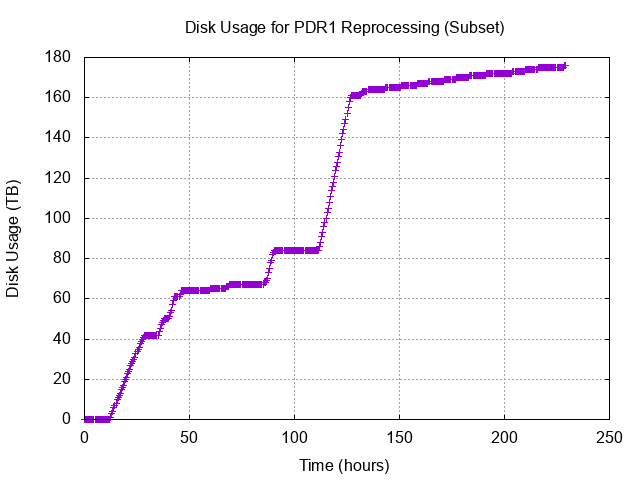
\includegraphics[width=0.45\textwidth]{figures/df_focus}
                 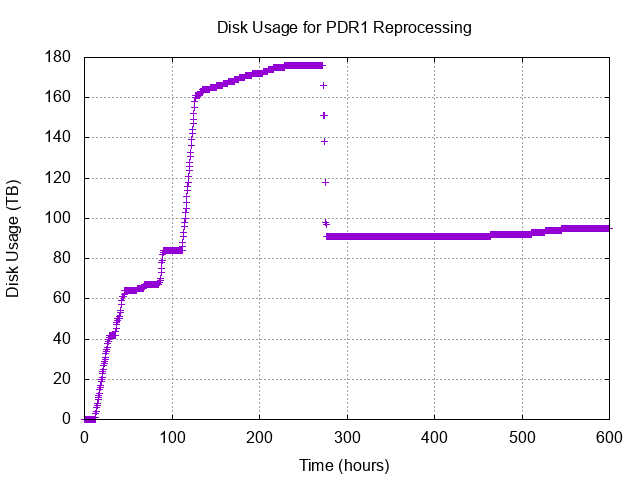
\includegraphics[width=0.45\textwidth]{figures/df}
                 \caption{Disk Usage of the production scratch space throughout the S17B reprocessing}
                 \label{fig:df}
        \end{center}
\end{figure}

The resultant data products are archived in 4 folders at /datasets/hsc/repo/rerun/DM-10404/. In total there are 11594219 files. The large files are typically hundreds of MBs.  The average size is ~14MB. The file size distribution is in Figure \ref{fig:file_size_dist}.

\begin{figure}[htbp]
        \begin{center}
                 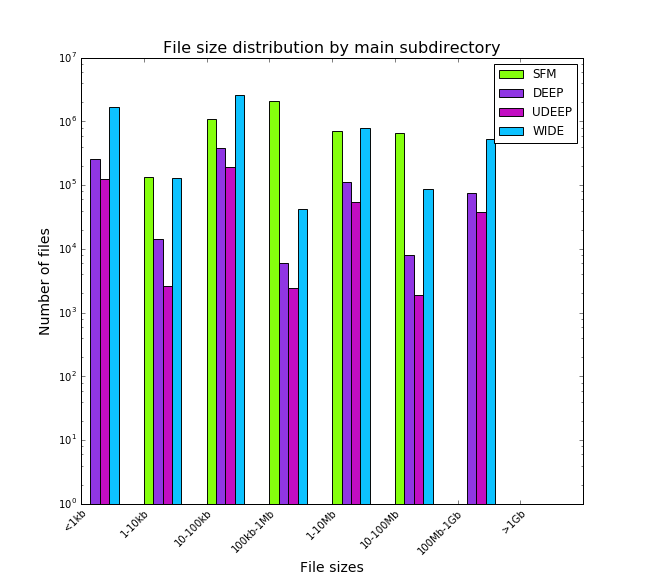
\includegraphics[width=\textwidth]{figures/file_size_dist}
                 \caption{file size distribution of the output repos}
                 \label{fig:file_size_dist}
        \end{center}
\end{figure}

Figure \ref{fig:butler_size} show the distributions for the data products in terms of butler dataset types.  All plots are in log scale.

\begin{figure}[htbp]
        \begin{center}
                 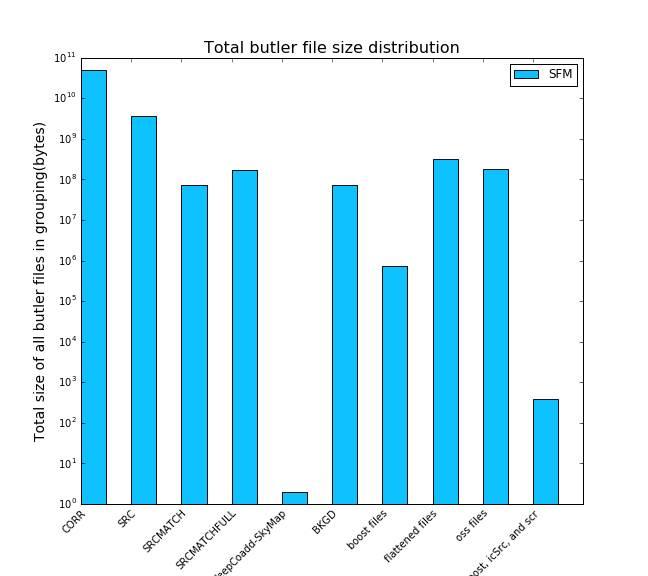
\includegraphics[width=0.7\textwidth]{figures/butler_size_sfm}
                 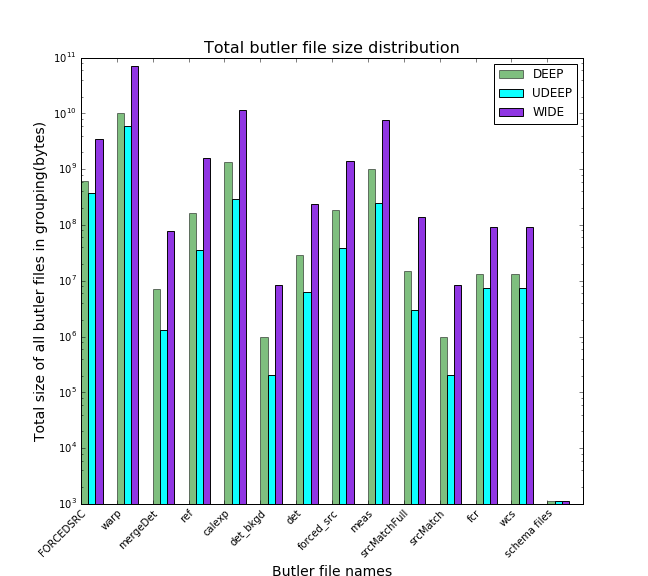
\includegraphics[width=0.7\textwidth]{figures/butler_size_duw}
                 \caption{Size distribution across butler types}
                 \label{fig:butler_size}
        \end{center}
\end{figure}

\subsection{CPU Usage}

The total CPU used was 79246 core-hours, that is, around 471.7 core-weeks.
The total User CPU was 76246 core-hours, that is, around 453.8 core-weeks.

The core-hours spent at each pipeline step were:
\begin{enumerate}
\item
sfm: 19596.9
\item
mosaic: 943.2
\item
coadd: 5444.9
\item
multiband: 34127.2
\item
forcedPhotCcd: 19133.9
\end{enumerate}
The percentage is shown in Figure \ref{fig:cpuPieChart}.

\begin{figure}[htbp]
        \begin{center}
                 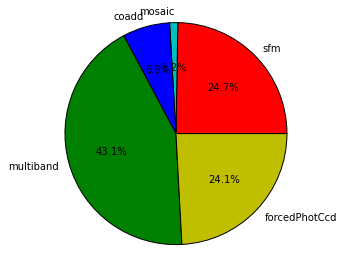
\includegraphics[width=0.6\textwidth]{figures/cpuPieChart}
                 \caption{CPU time for each pipeline}
                 \label{fig:cpuPieChart}
        \end{center}
\end{figure}

Figure \ref{fig:efficiency} shows the "efficiency", calculated by dividing the total cpu time by wall elapsed time * number of cores, for each pipeline.

\begin{figure}[htbp]
        \begin{center}
                 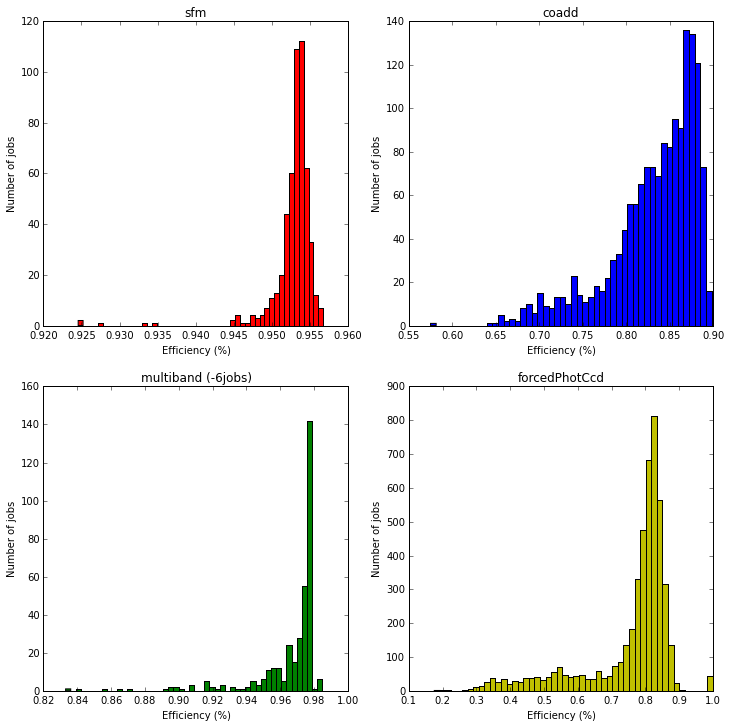
\includegraphics[width=\textwidth]{figures/efficiency}
                 \caption{Efficiency for each pipeline}
                 \label{fig:efficiency}
        \end{center}
\end{figure}

\begin{enumerate}
\item
A general feature of the plots is that the efficiency is observed to be bounded/limited by the fact that with ctrl{\_}pool/mpi the MPI root process is mostly idle and occupies one core.  This correlates with an upper bound for SFM of 23/24 ~0.958 , for coadd processing of 11/12 ~ 0.916, etc.

\item
sfm: Every 11 visits are grouped into one job, and each visit has 103 ccds. Thus, 1133 ccds were processed in a job, divided amongst 24 cores. Each ccd took around 2 minutes in average; in other words, roughly 90 min of wall clock elapsed time and 36 hr of accumulated CPU time per job. Efficiency is uniformly good. SingleFrameDriverTask is a ctrl{\_}pool BatchParallelTask.  The histogram below shows the CPU time of the SFM slurm jobs. The job IDs of the longest running jobs are: 51245, 51320, 51371, 51483, 51496, 51497, 51525, 51533, 51534, 51536, 51546, 51547, 51548, 51549, 51550, 51582, 51587, 51602, 51603
\begin{figure}[htbp]
        \begin{center}
                 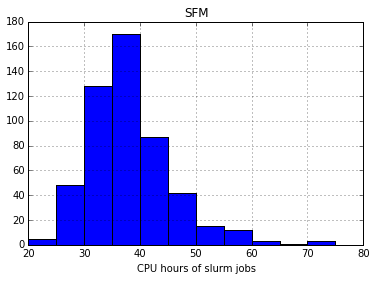
\includegraphics[width=0.6\textwidth]{figures/cpu_sfm}
                 \caption{CPU hours of the SFM pipeline}
                 \label{fig:cpu_sfm}
        \end{center}
\end{figure}

\item
mosaic: The unit of processing is each tract x filter on a node for each layer.  Mosaic jobs used 12 cores for reading source catalogs, via Python multiprocessing, but 1 core for other parts of the task; therefore we did not calculate the efficiency as it would be misleading. MosaicTask does not use ctrl{\_}pool.
\item
coadd: coadd jobs are chosen to process a tract on a node. One tract has 9*9=81 patches. CoaddDriverTask is a ctrl{\_}pool  BatchPoolTask. In most cases the patches are processed “12 wide” using ctrl{\_}pool, distributing the work to 12 cores on a node. Using mpi based ctrl{\_}pool in this context leads to one mostly idle MPI root process and 11 workers.  As Verification nodes have 128 GB RAM, this gives on average ~ 11 GB of memory per patch, with the aggregate  able to use the 128 GB.
\item
MultiBandDriver is a ctrl{\_}pool  BatchPoolTask.
Six multiband jobs (9476-mbWIDE9219, 59482-mbWIDE9737,59484-mbWIDE10050, 59485-mbWIDE10188,59486-mbWIDE16003, 59316-mbUDEEP8522) were excluded from this figure; their elapsed times were very short and had very bad efficiencies but they are from tracks outside of the survey coverage.
\item
Some of the forcedPhotCcd jobs run as only one task on one node had very high efficiency but this gave bad throughput.
\item
Figure \ref{fig:maxm} show the histograms of the maximum resident set size and the virtual memory size for mosaic and forcedPhotCcd. Memory Memory monitoring of ctrl{\_}pool driver jobs (singleFrameDriver, coaddDriver, multiBandDriver) was problematic and we do not believe in the numbers collected, so we do not plot them.

\begin{figure}[htbp]
        \begin{center}
                 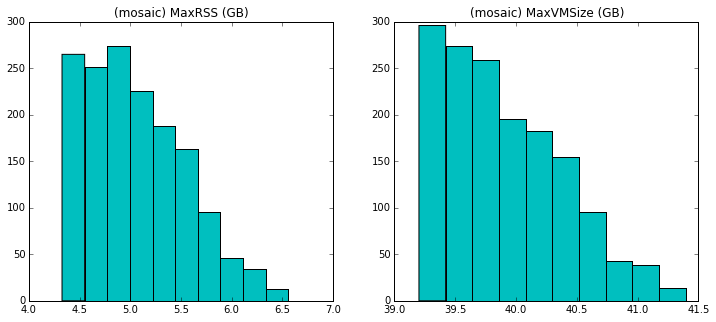
\includegraphics[width=\textwidth]{figures/maxm_mosaic}
                 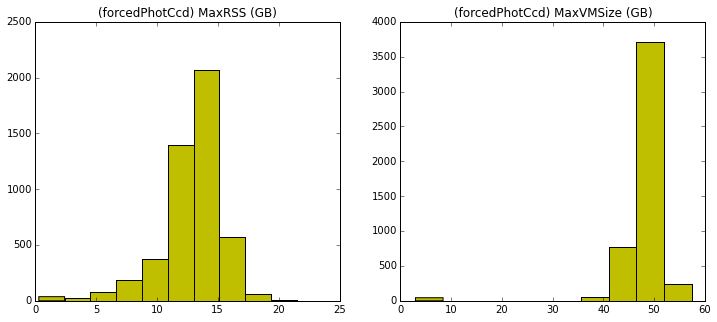
\includegraphics[width=\textwidth]{figures/maxm_forcPhotCcd}
                 \caption{Memory usage of mosaic and forcedPhotCcd pipelines}
                 \label{fig:maxm}
        \end{center}
\end{figure}

\end{enumerate}

\subsection{Node Utilization}

Figure \ref{fig:node} shows the node utilization throughout the campaign.
The Verification Cluster in its optimal state has 48 compute nodes with 24 physical cores, 128 GB RAM on each node.  For the duration of the S17B reprocessing there was a peak of 45 compute nodes available. The plot does not include failed jobs or test attempts, of which the generated data do not contribute to the final results directly.

\begin{figure}[htbp]
        \begin{center}
                 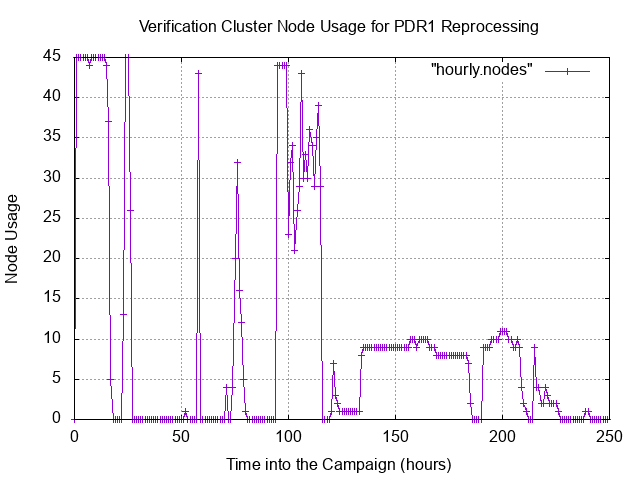
\includegraphics[width=\textwidth]{figures/nodeUtilization}
                 \caption{hourly node usage \label{fig:node}}
        \end{center}
\end{figure}

\section{Triggered JIRA tickets}
Some of the stack issues identified during the S17B Reprocessing
have been turned into actionable JIRA tickets.
Tickets for Science Pipelines improvements are
\jira{DM-10574} (Hit AssertionError in deblender),
\jira{DM-10755} (forcedPhotCcd.py fails with the non-existing reference of a barely-overlapping patch),
\jira{DM-10782} (Add bright star masks to ci{\_}hsc), and
\jira{DM-10413} (Please complain louder if brightObjectMask cannot be found).
Tickets for Middleware improvements are
\jira{DM-10761} (Failed CmdLineTask does not give nonzero exit code; resolved by \jira{}),
\jira{DM-10624} (Duplicate log files from running pipe{\_}drivers tasks), and
\jira{DM-11171} (Please separate algorithmic configs and operational configs in the task framework).

Many of the low-level processing issues are related to either the task framework design or the Data Butler.
Issues related to the framework design were not turned into JIRA tickets,
but concerns were brought to the SuperTask Working Group and Butler Working Group.


% Include all the relevant bib files.
% https://lsst-texmf.lsst.io/lsstdoc.html#bibliographies
\bibliography{lsst,lsst-dm,refs_ads,refs,books,local}

\end{document}
